\documentclass[runningheads]{llncs}
%
\usepackage[T1]{fontenc}
% T1 fonts will be used to generate the final print and online PDFs,
% so please use T1 fonts in your manuscript whenever possible.
% Other font encondings may result in incorrect characters.
%
\usepackage{graphicx}
% Used for displaying a sample figure. If possible, figure files should
% be included in EPS format.
%
% If you use the hyperref package, please uncomment the following two lines
% to display URLs in blue roman font according to Springer's eBook style:
%\usepackage{color}
%\renewcommand\UrlFont{\color{blue}\rmfamily}

\usepackage{amsmath}
\usepackage{amssymb}    % for \rightsquigarrow
\usepackage{wasysym}	% for frown face
\usepackage{mathrsfs} 	% for \mathscr
\usepackage{stmaryrd}
\usepackage{mathtools}		% to extend length of double harpoon arrows

\begin{document}
%
\title{AGI from the perspectives of Categorical Logic and Algebraic Geometry}
%
%\titlerunning{Abbreviated paper title}
% If the paper title is too long for the running head, you can set
% an abbreviated paper title here
%
\author{King-Yin Yan \orcidID{0009-0007-8238-2442}}
%
\authorrunning{K-Y. Yan}
% First names are abbreviated in the running head.
% If there are more than two authors, 'et al.' is used.
%
\institute{\email{general.intelligence@gmail.com}}
%
\maketitle              % typeset the header of the contribution
%
\begin{abstract}
To ``situate'' AGI in the context of current mathematics, so that mathematics-minded professionals can more easily see whether current mathematical ideas can be fruitfully applied to AGI.

\keywords{AGI  \and categorical logic \and homotopy type theory \and Curry-Howard isomorphism \and algebraic geometry.}
\end{abstract}
%
%
%
\section{Goal of this paper}

The bottleneck of AGI development is the speed of learning algorithms.  The cost of training GPT-4 was rumored to be \$100M (by Sam Altman).  To speed up learning, one needs to introduce inductive biases, according to the No Free Lunch theorem.  One principled way to introduce inductive bias is by imposing the structure of logic.  One reasons that, if humans have discovered the structure of logic in this world, an intelligent program may re-discover the same structure.  So our question is:  what is the mathematical structure of logic?

Traditionally this line of research is called algebraic logic, starting from Leibniz and Boole, up to more recent times Tarski's cylindrical algebra and Paul Halmos' work.  

\section{Our conclusions so far}

The conclusions of this paper are mostly negative.  That is, the mathematical structures described here seem unable to offer practical ways to accelerate AGI, unless the reader can discover more ingenious ideas.  Nevertheless we hope the presentation of the ideas thus far can help the readers on their way.

\subsection{Basic categorical logic}

\subsection{Modal logic}

\subsection{Homotopy type theory}

\subsection{Algebraic geometry}

The fundamental duality in algebraic geometry is:
\begin{equation}
\left\{ \begin{tabular}{cc} spaces, or \\ varieties \end{tabular} \right\} \longleftrightarrow \left\{ \begin{tabular}{cc} commutative \\ $\mathbf{k}$-algebras \end{tabular} \right\}
\end{equation}
within this correspondence, we have:
\begin{equation}
\left\{ \begin{tabular}{cc} points in \\ geometry \end{tabular} \right\} \longleftrightarrow \left\{ \begin{tabular}{cc} prime ideals \end{tabular} \right\}
\end{equation}

An approach suggested by Yuri Manin is to turn logic into an algebra, such as the Boolean ring (but this can only handle propositional logic).  Varieties defined by such Boolean polynomials \cite{ref_article1} live in the space $\mathbb{Z}_2^n$, the discrete hypercube.  

My visualization of the ``Grothendieck picture'' of AGI is like this:
\begin{equation}
\vcenter{\hbox{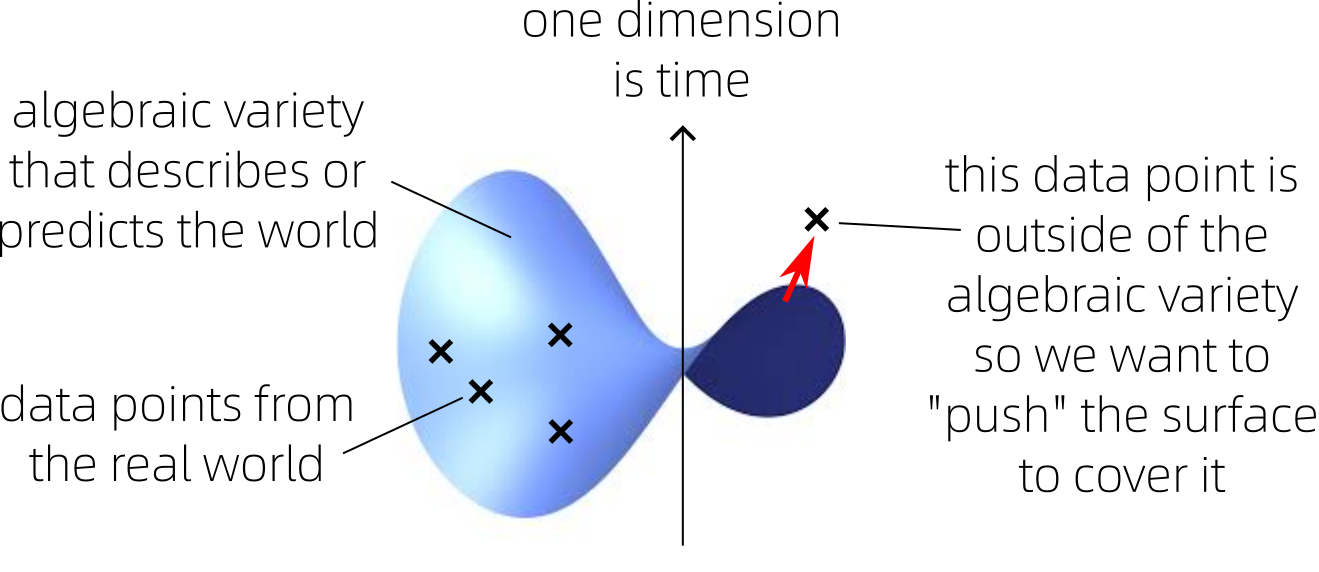
\includegraphics[scale=0.7]{Grothendieck-picture.png}}} \nonumber
\end{equation}

One of the interesting discoveries in categorical logic is that every topos admits an \textbf{internal language}.  This is a simple consequence of Curry-Howard: since a type-space corresponds to a logic proposition, and categorical logic interprets a type-space as an object in the category, thus every category (satisfying extra conditions) can be interpreted as having an ``internal'' logic.  The converse of this correspondence is the \textbf{classifying topos} of a logic theory:
\begin{equation}
\underset{\footnotesize\text{classifying topos}}{\mathcal{E}_\mathbb{T}} \xrightleftharpoons[]{\; \text{ internal language } \;} \underset{\footnotesize\text{theory}}{\mathbb{T}}
\end{equation}

\begin{equation}
\vcenter{\hbox{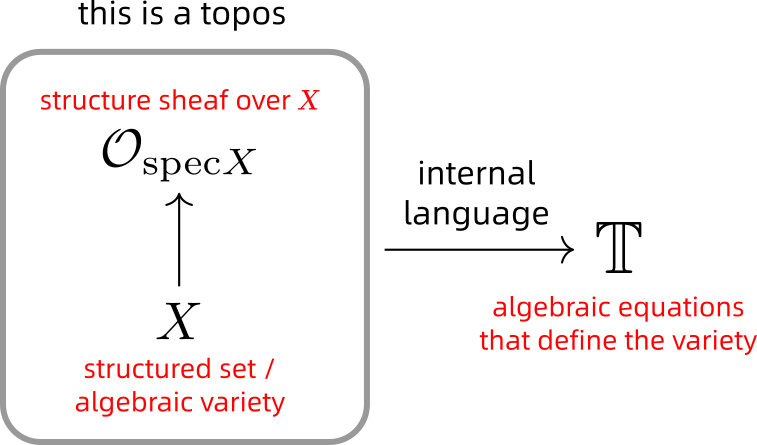
\includegraphics[scale=0.8]{geometric-topos.png}}}
\end{equation}

% 代数几何中最特别的地方是出现了 由代数方程 =0 定义的代数簇,这个带结构的空间 与抽象的 scheme 对应,scheme 是研究代数簇的更抽象而合理的对象。 范畴逻辑来自 Curry-Howard 的传统,我研究的目的是寻找 逻辑在数学中的适当位置,但也寻找逻辑的更 general 形式。 逻辑加入了「数量」运算之后,可以处理「方程」的问题,而在另一方向发展,它处理自然语言的问题。

\begin{table}
\caption{Table captions should be placed above the
tables.}\label{tab1}
\begin{tabular}{|l|l|l|}
\hline
Heading level &  Example & Font size and style\\
\hline
Title (centered) &  {\Large\bfseries Lecture Notes} & 14 point, bold\\
1st-level heading &  {\large\bfseries 1 Introduction} & 12 point, bold\\
2nd-level heading & {\bfseries 2.1 Printing Area} & 10 point, bold\\
3rd-level heading & {\bfseries Run-in Heading in Bold.} Text follows & 10 point, bold\\
4th-level heading & {\itshape Lowest Level Heading.} Text follows & 10 point, italic\\
\hline
\end{tabular}
\end{table}

\begin{figure}
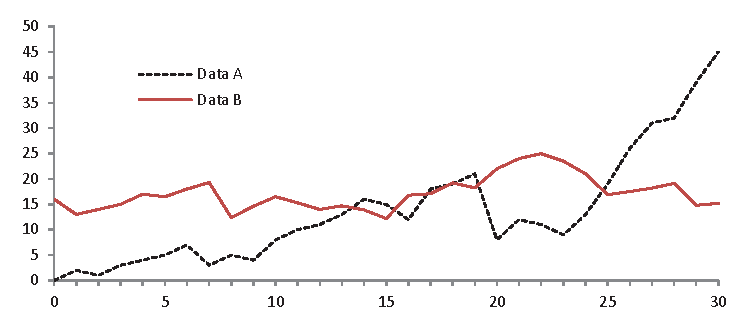
\includegraphics[width=\textwidth]{fig1.eps}
\caption{A figure caption is always placed below the illustration.
Please note that short captions are centered, while long ones are
justified by the macro package automatically.} \label{fig1}
\end{figure}

\begin{theorem}
This is a sample theorem. The run-in heading is set in bold, while
the following text appears in italics. Definitions, lemmas,
propositions, and corollaries are styled the same way.
\end{theorem}
%
% the environments 'definition', 'lemma', 'proposition', 'corollary',
% 'remark', and 'example' are defined in the LLNCS documentclass as well.
%

\subsubsection{Acknowledgements} Please place your acknowledgments at
the end of the paper, preceded by an unnumbered run-in heading (i.e.
3rd-level heading).

%
% ---- Bibliography ----
%
% BibTeX users should specify bibliography style 'splncs04'.
% References will then be sorted and formatted in the correct style.
%
% \bibliographystyle{splncs04}
% \bibliography{mybibliography}
%
\begin{thebibliography}{8}
\bibitem{ref_article1}
Author, F.: Article title. Journal \textbf{2}(5), 99--110 (2016)

\bibitem{ref_lncs1}
Author, F., Author, S.: Title of a proceedings paper. In: Editor,
F., Editor, S. (eds.) CONFERENCE 2016, LNCS, vol. 9999, pp. 1--13.
Springer, Heidelberg (2016). \doi{10.10007/1234567890}

\bibitem{ref_book1}
Author, F., Author, S., Author, T.: Book title. 2nd edn. Publisher,
Location (1999)

\bibitem{ref_proc1}
Author, A.-B.: Contribution title. In: 9th International Proceedings
on Proceedings, pp. 1--2. Publisher, Location (2010)

\bibitem{ref_url1}
LNCS Homepage, \url{http://www.springer.com/lncs}. Last accessed 4
Oct 2017
\end{thebibliography}
\end{document}
